\chapter{Validazione in ambiente reale}
\label{cap:campo}

% ---------------------------------------------------------------------
% CAPITOLO NUOVO, non presente nella bozza iniziale.
% Nasce dalla richiesta esplicita del relatore di provare il sistema con
% una sessione lunga in una casa vera.
%
% Scritto il 2026-08-17, a sessioni eseguite. La sezione 6.2 contiene una
% previsione formulata PRIMA della prima sessione (EXP-032) e va letta
% come tale: e' il termine di paragone di tutto il capitolo.
%
% Fonti: EXP-032, EXP-036, EXP-043, EXP-044, EXP-047..EXP-054,
% ISS-036, ISS-040, ISS-042, docs/PROTOCOLLO_SESSIONE_REALE.md
% ---------------------------------------------------------------------

I capitoli precedenti hanno validato il sistema \emph{in vitro}: dieci soggetti, una stanza di laboratorio, cadute recitate su un materasso, annotazione fotogramma per fotogramma. Nessuna delle metriche prodotte finora dice cosa succede lasciando il sistema acceso per ore in una casa dove nessuno cade.

Questo capitolo risponde a quella domanda, e il risultato principale non è un numero di prestazione: è che \textbf{l'insieme di verifica su cui l'intero settore misura ordina in modo errato le alternative progettuali}.

\section{Perché il laboratorio non basta}
\label{sec:perche-non-basta}

Il divario fra prestazioni dichiarate e comportamento sul campo non è un'ipotesi di questo lavoro: è un fenomeno documentato. Bagalà e colleghi hanno preso tredici algoritmi di rilevamento cadute pubblicati, che dichiaravano sensibilità comprese fra il 76\% e il 100\% su cadute simulate, e li hanno rieseguiti su un archivio di ventinove cadute reali confermate. La sensibilità media misurata è stata del \textbf{57,0\%} con una dispersione di 27,3 punti, e i falsi allarmi in ventiquattro ore di monitoraggio andavano da cinque a ottantacinque al giorno a seconda dell'algoritmo.

Il fenomeno è stato riconfermato di recente e su scala molto maggiore. Il benchmark OmniFall unifica otto dataset pubblici di rilevamento cadute --- fra cui UP-Fall --- per circa ottanta ore annotate a livello di fotogramma, e li confronta con un insieme di cadute \emph{vere} riprese fuori dal laboratorio. Il modello addestrato su UP-Fall passa da un F1 di 72,9\% in dominio a \textbf{16,9\%} sulle cadute reali; su Le2i il crollo è da 100\% a 58,8\%. E il collo di bottiglia identificato è proprio la distinzione fra \emph{fallen} e \emph{lying}: i modelli confondono sistematicamente chi è caduto con chi è disteso.

Ci sono due ragioni per cui un dataset di laboratorio non può misurare ciò che serve, e sono di natura diversa.

La prima è la \textbf{frequenza di base}, ed è quantificabile a priori: è la sezione~\ref{sec:frequenza-base}.

La seconda è più insidiosa perché non si vede finché non si va a misurare: il dataset \textbf{non contiene le situazioni difficili} dell'ambiente di destinazione. UP-Fall non ha divani, non ha più persone in scena, e --- come si vedrà --- le sue persone orizzontali che non sono cadute stanno a terra invece che rialzate. Ogni intervento progettato per una condizione che il dataset non rappresenta viene giudicato da quel dataset come un peggioramento.

\section{Il problema della frequenza di base}
\label{sec:frequenza-base}

Questa sezione è stata scritta \emph{prima} della prima sessione, ed è importante che si legga in quest'ordine: contiene una previsione, e una previsione registrata dopo i fatti non è una previsione.

Il modello migliore del Capitolo~\ref{cap:risultati} produce circa 46 falsi positivi su 4.767 finestre negative, cioè lo \textbf{0,96\% per finestra}. In laboratorio, dove le finestre positive sono il 4,5\% del totale, quello 0,96\% corrisponde a una precision di 0,819 --- un numero che si presenta bene.

In un soggiorno la quota di finestre positive è circa lo zero per cento. Proiettando lo stesso tasso per finestra sul funzionamento continuo:

\begin{center}
\begin{tabular}{lrr}
\toprule
Modalità di finestratura & Finestre/giorno & Falsi allarmi/giorno \\
\midrule
Finestre non sovrapposte & $\sim$34.560 & $\sim$332 \\
Finestre con stride 5 & $\sim$311.000 & $\sim$2.990 \\
\bottomrule
\end{tabular}
\end{center}

Cioè fra \textbf{14 e 125 falsi allarmi all'ora}.

Il punto metodologico è che \textbf{la precision non è una proprietà del modello}: dipende da quanto sono frequenti gli eventi positivi nell'insieme su cui la si calcola. Riportare una precision misurata su un insieme quasi bilanciato come se descrivesse il comportamento in esercizio è un errore diffuso in letteratura, e qui viene quantificato con dati propri.

Il termine di paragone esterno rende la distanza esplicita. Il criterio che circola come soglia di accettabilità clinica è rilevare almeno il 95\% delle cadute con al massimo \textbf{uno o due falsi allarmi alla settimana}. I sistemi realmente installati e documentati riportano 73\% di sensibilità con un falso allarme ogni quarantasei giorni, oppure 80\% con uno ogni venti giorni --- e nel primo caso una precision del 37,5\%, in un sistema considerato funzionante. Fra la previsione di 14--125 allarmi all'ora e il bersaglio di uno o due alla settimana ci sono \textbf{tre o quattro ordini di grandezza}, e non si colmano migliorando il classificatore.

\section{Protocollo delle sessioni}
\label{sec:protocollo-campo}

Sono stati registrati \textbf{dodici blocchi in quattro giornate, in due abitazioni, per 9,6 ore complessive}. I partecipanti sono familiari dello studente, informati e consenzienti; il relatore è stato informato della natura della raccolta.

La telecamera è montata \textbf{lateralmente} a 1,5--2~m di altezza. Non è una scelta di comodo: discende direttamente dal risultato del Capitolo~\ref{cap:risultati}, dove il passaggio da una vista laterale a una frontale rialzata dimezza l'accuratezza.

I blocchi si dividono in tre tipi:

\begin{itemize}
  \item \textbf{vita normale}, che fornisce il denominatore dei falsi allarmi ed è l'unico tipo registrato a casa dei nonni;
  \item \textbf{cadute recitate}, con orari annotati dall'operatore, che fornisce il recall;
  \item \textbf{trappole}, cioè attività costruite per far sbagliare il sistema: sdraiarsi sul divano, sedersi di scatto, chinarsi, stare a terra volontariamente, più persone in campo.
\end{itemize}

\paragraph{Etica e privacy come contenuto, non come adempimento.} Il registratore scritto per queste sessioni salva in modo continuo \emph{soltanto posa e feature}: mai il video. Le immagini vengono conservate solo in una finestra di pochi secondi attorno agli allarmi, restano sul dispositivo e non entrano nel repository. È il \emph{privacy-by-design} argomentato nel Capitolo~\ref{cap:contesto} dimostrato in pratica invece che dichiarato --- e ha richiesto di rimuovere dal prototipo una registrazione video continua che era stata aggiunta per comodità di sviluppo e che contraddiceva l'argomento stesso della tesi.

Una scelta va dichiarata perché limita i risultati: \textbf{i partecipanti anziani non eseguono cadute recitate}. Nei loro blocchi c'è soltanto vita normale. La ragione è di sicurezza, e la conseguenza è che il recall non è mai misurato sulla popolazione a cui il sistema sarebbe destinato.

\section{La prima ora, e cosa ha cambiato}
\label{sec:prima-ora}

Il primo blocco è durato trentanove minuti e ha prodotto \textbf{2.735 allarmi all'ora}: \textbf{ventidue volte} il limite superiore della previsione della sezione~\ref{sec:frequenza-base}. Una previsione costruita per essere scomoda si è rivelata ottimistica di oltre un ordine di grandezza.

Il dato che spiega il meccanismo è la distribuzione nel tempo:

\begin{center}
\begin{tabular}{lrr}
\toprule
Minuti & Pose valide & Allarmi \\
\midrule
0--15 (stanza vuota) & 0--29\% & \textbf{0} \\
15--25 & 76\% & 105--124 \\
25--35 & 76--99\% & 454--462 \\
35--40 (cadute) & 81\% & 642 \\
\bottomrule
\end{tabular}
\end{center}

\textbf{Zero allarmi in quindici minuti di stanza vuota.} Il problema non è rumore di fondo: è che ogni movimento di una persona presente genera finestre positive, e a finestre sovrapposte un singolo evento ne produce decine.

\section{Falsi allarmi in funzionamento continuo}
\label{sec:falsi-allarmi}
\label{sec:finestre-eventi}

Nella sessione da cinque ore, dopo aver alzato la soglia, il tasso scende a 41,7 finestre sopra soglia all'ora, che diventano \textbf{3,41 allarmi all'ora contando gli eventi} invece delle singole finestre. È un miglioramento di quasi tre ordini di grandezza rispetto alla prima ora, ed è ancora un ordine di grandezza sopra gli 0,4 all'ora delle installazioni funzionanti documentate, e due o tre sopra il criterio clinico.

La terza sessione, a casa dei nonni, ha dato \textbf{1.635 allarmi all'ora}: \textbf{trentanove volte} la casa precedente, a parità di configurazione, di soglia e di stimatore. La causa è stata osservata direttamente sui fotogrammi conservati attorno agli allarmi: \textbf{due persone anziane distese su due divani, immobili, nel pomeriggio}. Non è un caso limite costruito per mettere in difficoltà il sistema; è la loro vita normale, ed è esattamente la popolazione a cui il sistema sarebbe destinato.

\paragraph{Il filtro temporale non basta, e la ragione è strutturale.} La logica di soppressione delle raffiche --- richiedere $N$ finestre consecutive sopra soglia e poi sospendere per un periodo --- è progettata per \emph{eventi}. Una persona distesa per un'ora non è un evento ma uno \emph{stato che dura}, e fa riscattare l'allarme a ogni scadenza del periodo di sospensione. Il filtro comprime le raffiche e non gli stati, e in una casa con anziani il falso positivo dominante è uno stato.

\subsection{Finestre contro eventi}

Prima di ogni altra cosa va fissata l'unità di misura, perché è all'origine di
gran parte dei numeri irriportabili di questo capitolo.

Il sistema produce una decisione ogni frazione di secondo. Una singola caduta
genera quindi una \emph{raffica} di finestre consecutive sopra soglia --- su
una delle sessioni registrate una sola caduta ne ha prodotte centoventinove ---
e contarle come altrettanti allarmi non è una semplificazione: è un errore di
un fattore misurato in \textbf{47,8}.

Un allarme è definito da due parametri dichiarati: \textbf{cinque finestre
consecutive} sopra soglia perché venga emesso, e \textbf{trenta secondi} di
sospensione dopo l'emissione. Ogni numero di questo capitolo espresso in
«eventi all'ora» adotta questa regola; i numeri espressi in «finestre all'ora»
la precedono, e i due non vanno confrontati fra loro né con la letteratura,
che riporta eventi.

\subsection{La definizione del compito, misurata in casa}

La diagnosi del paragrafo precedente --- il falso positivo dominante è uno
stato che dura, e nessun filtro temporale comprime uno stato --- contiene già
la soluzione, ma in una direzione che non è quella del filtro. Se lo stato è
il problema, il sistema non deve riconoscere lo stato.

I tre compiti definiti nel Capitolo~\ref{cap:metodologia} sono stati quindi
misurati sulle stesse registrazioni domestiche, con la stessa regola di
allarme e la stessa soglia:

\begin{center}
\begin{tabular}{lrr}
\toprule
Compito & Eventi/ora & Cadute rilevate \\
\midrule
\textbf{evento} --- la transizione & \textbf{1,6} & 3/5 \\
stato --- persona a terra & 29,5 & 0/5 \\
allarme --- l'uno o l'altro & 36,4 & 4/5 \\
\bottomrule
\end{tabular}
\end{center}

\textbf{Un fattore ventitré sui falsi allarmi, al costo di una caduta su
cinque.} Il compito \emph{stato}, che è la formulazione più diffusa in
letteratura, è anche l'unico che in queste registrazioni non rileva alcuna
caduta: riconosce la persona distesa sul divano e quella caduta a terra come
la stessa configurazione, e alla soglia dichiarata satura sui divani.

Il dato è coerente con quanto misurato in laboratorio nella
sezione~\ref{sec:compito-risultati}, dove il compito \emph{evento} sbaglia
sullo zero per cento delle finestre di persona distesa volontariamente. Che la
stessa scelta produca lo stesso ordine in due contesti così diversi è la
corroborazione più solida di cui questo lavoro disponga.

\paragraph{Che cosa questo \emph{non} risolve.} Un evento e mezzo all'ora resta
lontano dagli $0{,}05$ delle installazioni documentate, di un fattore trenta. E
il compito \emph{evento} paga il proprio vantaggio esattamente dove costa di
più: una caduta non rilevata su cinque. La direzione è giusta, la distanza dal
requisito clinico non è colmata.


\begin{figure}[ht]
\centering
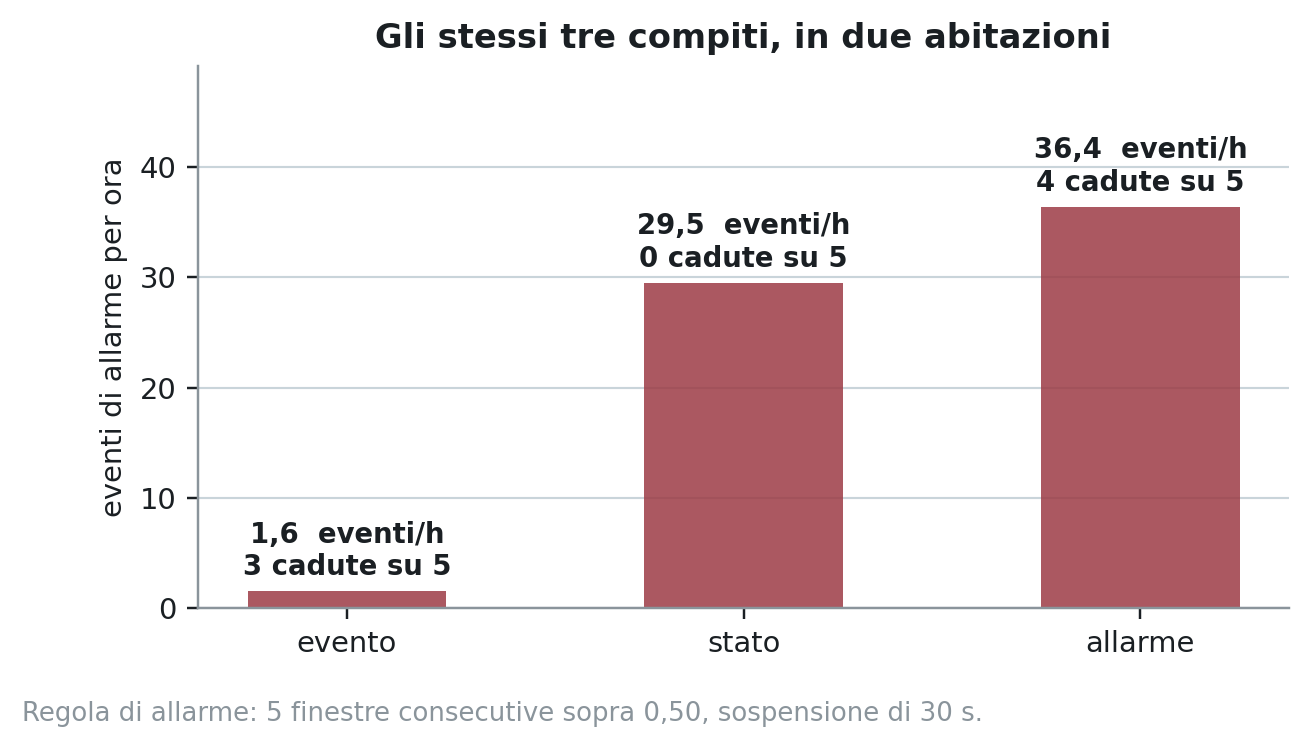
\includegraphics[width=.76\textwidth]{figure/fig_compiti_casa.png}
\caption{Gli stessi tre compiti misurati sulle registrazioni domestiche, con la regola di allarme dichiarata: cinque finestre consecutive sopra soglia e trenta secondi di sospensione. Il compito \emph{evento} è l'unico compatibile con un uso continuativo. Prodotta da \texttt{pipeline/figure\_tesi.py} sui risultati a dieci soggetti.}
\label{fig:compiti-casa}
\end{figure}

\section{Recall fuori dal laboratorio}
\label{sec:recall-campo}

Sulle cinque cadute annotate della sessione dedicata, la configurazione di riferimento ne rileva quattro.

Il numero va però letto con tre riserve, e la terza è emersa solo ricontando gli allarmi nel modo in cui li conterebbe chi usa il sistema.

La prima è la numerosità: \textbf{cinque cadute} non stimano un recall, danno un indizio. La seconda è che in quella sessione l'inquadratura era difettosa, con il corpo che esce dal bordo inferiore dell'immagine in quattro casi su cinque.

\paragraph{La terza: quel «quattro su cinque» conta finestre, non allarmi.} Un sistema installato non produce finestre ma \emph{eventi}: una caduta o viene segnalata o no, e una raffica di finestre consecutive sopra soglia è un allarme, non cento. Ricontando per evento, il recall dipende da due parametri dell'analisi che non erano stati dichiarati --- la \textbf{tolleranza di accoppiamento}, cioè entro quanto tempo dalla caduta annotata un allarme conta come rilevamento, e la \textbf{persistenza}, cioè quante finestre consecutive sopra soglia servono perché l'allarme scatti.

\begin{center}
\begin{tabular}{lcc}
\toprule
Tolleranza & Persistenza 1 & Persistenza 5 \\
\midrule
$\pm 10$~s & 0/4 & 0/4 \\
$\pm 30$~s & 2/5 & 1/5 \\
$\pm 60$~s & 3/5 & 1/5 \\
$\pm 90$~s & \textbf{4/5} & 1/5 \\
\bottomrule
\end{tabular}
\end{center}

Il valore riportato finora si colloca nell'angolo \emph{più permissivo} della tabella: una banda di tre minuti attorno alla caduta e un allarme che scatta su una singola finestra. Con parametri clinicamente difendibili --- l'allarme entro mezzo minuto e non su una finestra isolata --- il recall è \textbf{una caduta su cinque}.

La tolleranza larga non è sostenibile per due ragioni. L'annotazione dell'operatore è al minuto, quindi l'istante vero è noto a meno di sessanta secondi e $\pm 30$~s è già generoso; e in una sessione che produce centinaia di finestre sopra soglia all'ora, in una banda di tre minuti un allarme si trova quasi sempre, e viene attribuito alla caduta anche quando è stato causato da altro. Contraddice inoltre la motivazione clinica del Capitolo~\ref{cap:contesto}: se il danno dipende dal tempo passato a terra, un allarme novanta secondi dopo non è un rilevamento tempestivo.

Sullo stesso criterio è stato ricontato l'archivio esterno: su venti riprese di caduta di UR-Fall il sistema non ne segnala \textbf{nessuna}. Il conteggio per finestra ne dava nove su 144; per evento dà zero, perché i punteggi si fermano appena sotto la soglia e non vi restano abbastanza a lungo.

\paragraph{Il terzo parametro implicito.} È la terza volta in questo lavoro che un numero di intestazione dipende da un'impostazione dell'analisi lasciata come costante: dopo il sottocampionamento applicato alle sessioni e la media dei modelli della validazione incrociata al posto di quello installato, ora la tolleranza e la persistenza. Tutte e tre nella direzione che migliora il risultato, e nessuna per scelta deliberata --- sono impostazioni ereditate da uno script all'altro. Il rimedio adottato è esporle come parametri e riportare il recall di campo come \textbf{intervallo con i parametri dichiarati}, mai come numero singolo.

\paragraph{Un errore di misura che andava trovato prima di ogni confronto.} La valutazione fuori linea dava inizialmente 2 cadute su 5 dove la board, sugli stessi eventi e con lo stesso modello, ne aveva segnalate 4. Due procedure che guardano gli stessi dati non possono dare risultati diversi, e finché la discrepanza non è stata spiegata nessun confronto fra configurazioni era valido.

Le cause erano due. La prima, minore: fuori linea si mediavano i modelli della validazione incrociata, ciascuno addestrato su un sottoinsieme dei soggetti, mentre sul dispositivo gira un modello addestrato su tutti. La seconda, decisiva: l'analisi applicava alle sessioni lo stesso sottocampionamento usato su UP-Fall --- un fotogramma su due, per portare i 18~fps del dataset ai 9 su cui il modello è addestrato --- ma \textbf{le sessioni sulla board girano già a 7--8~fps}, e dimezzarle le porta a quattro. La finestra da 22 campioni copriva così cinque secondi e mezzo invece di due e mezzo, e la caduta ci si perdeva dentro.

È lo stesso difetto già trovato e risolto sul lato hardware, ricomparso \textbf{dal lato opposto della catena}: introdotto dall'analisi invece che dal dispositivo. Corrette entrambe le cause, la configurazione di riferimento dà 4 su 5, esattamente come la board.

\section{Che cosa il laboratorio non riesce a misurare}
\label{sec:rovesciamento}

È il risultato centrale del capitolo e, si sostiene qui, dell'intera tesi.

Tre interventi sono stati progettati per la robustezza in ambiente domestico:
l'altezza del bacino rispetto al pavimento stimata automaticamente
(\emph{A3h}); l'inserimento in addestramento di controesempi ricavati dalle
sessioni senza cadute; e le grandezze integrali al posto delle derivate
istantanee (\emph{A3i}). Tutti e tre sono stati valutati con la \emph{stessa}
procedura, sugli \emph{stessi} modelli, su due insiemi di verifica diversi:
la validazione incrociata su dieci soggetti di laboratorio, e sette ore di
registrazione continua in due abitazioni.

\begin{center}
\begin{tabular}{lrrr}
\toprule
Configurazione & $F_2$ laboratorio & Finestre/ora in casa & Cadute \\
\midrule
A3 --- riferimento & $0{,}898 \pm 0{,}075$ & 139,9 & 3/5 \\
A3h --- con l'altezza & $0{,}931 \pm 0{,}051$ & 70,4 & 2/5 \\
A3h + controesempi & $0{,}942 \pm 0{,}060$ & \textbf{2,1} & 2/5 \\
A3i --- con gli integrali & $0{,}943 \pm 0{,}064$ & 9,8 & \textbf{4/5} \\
\textbf{A3i + controesempi} & $\mathbf{0{,}953 \pm 0{,}055}$ & 2,7 & 3/5 \\
\bottomrule
\end{tabular}
\end{center}

\paragraph{Una precisazione sull'unità.} La colonna centrale conta
\textbf{finestre} sopra soglia per ora, non eventi di allarme. Le due
grandezze differiscono di quasi due ordini di grandezza, e la
sezione~\ref{sec:finestre-eventi} le distingue: qui si usano le finestre
perché è la grandezza su cui le cinque configurazioni sono direttamente
confrontabili, non perché sia quella da riportare.

\subsection{Le due graduatorie concordano. Non è questo il punto}

Va detto subito, perché una versione precedente di questo lavoro sosteneva il
contrario. Con cinque soggetti la configurazione A3h con i controesempi
risultava la \emph{peggiore} in laboratorio ($F_2 = 0{,}780$) e quasi la
migliore in casa, e se ne era tratto un rovesciamento dell'ordine. Con dieci
soggetti quella stessa configurazione ottiene $0{,}942$, e \textbf{le due
graduatorie non si contraddicono}: la configurazione peggiore in laboratorio è
anche la peggiore in casa.

Il rovesciamento era in larga parte un effetto della scarsità di dati. Averlo
scritto e poi smentito è, nell'economia di questo lavoro, un episodio della
stessa storia che il Capitolo~\ref{cap:protocollo} racconta: una differenza
più piccola della dispersione fra soggetti non è una differenza, e con cinque
persone $0{,}780$ e $0{,}917$ non lo erano.

\subsection{Il laboratorio non ordina male: non risolve}

La conclusione che sostituisce il rovesciamento si legge confrontando le due
colonne per \emph{ampiezza}, non per ordine.

\begin{center}
\begin{tabular}{lrr}
\toprule
Da A3 ad A3i + controesempi & In laboratorio & In casa \\
\midrule
Variazione & $+0{,}055$ di $F_2$ & da 139,9 a 2,7 finestre/ora \\
Rapporto & --- & \textbf{52$\times$} \\
Confronto con il rumore & \textbf{dentro} la dispersione ($\pm 0{,}06$--$0{,}08$) & --- \\
\bottomrule
\end{tabular}
\end{center}

\textbf{La stessa coppia di configurazioni differisce di un fattore
cinquantadue in una casa e di una quantità indistinguibile dal rumore in
laboratorio.} Il dataset di riferimento non sbaglia l'ordine: comprime una
differenza enorme in una differenza che non si può dichiarare.

L'effetto pratico è identico a quello di un ordinamento errato. Chi selezioni
la configurazione sulla base del solo $F_2$ di laboratorio non ha alcuna
ragione statistica per preferire A3i con i controesempi ad A3 di riferimento:
le due sono indistinguibili, e la seconda è più semplice. Sceglierebbe quindi
la più semplice, e installerebbe un sistema che produce cinquantadue volte i
falsi allarmi.

\subsection{La causa è misurabile, non congetturale}

In entrambi gli insiemi esistono persone orizzontali che non sono cadute, ma
sono di tipo opposto.

\begin{center}
\begin{tabular}{lrl}
\toprule
Negativi orizzontali & Quota & Dove stanno \\
\midrule
Archivio di laboratorio & circa un quinto & a terra \\
Sessioni domestiche & circa metà & su una superficie rialzata \\
\bottomrule
\end{tabular}
\end{center}

In laboratorio sdraiarsi sul pavimento è una delle azioni registrate come
attività ordinaria: lì «corpo a terra» non discrimina, perché a terra ci si
trova sia dopo una caduta sia per scelta. In una casa chi è orizzontale senza
essere caduto sta quasi sempre su un divano o su un letto, e la distinzione fra
divano e pavimento è esattamente quella che serve --- ed è quella che
l'archivio, non avendo divani, non può premiare.

Se ne ricava un enunciato che si ritiene valga oltre il caso particolare:

\begin{quote}
Un insieme di verifica non può misurare un miglioramento su una condizione che
non rappresenta. Non si limita a sovrastimare le prestazioni: \textbf{rende
indistinguibili alternative che in esercizio differiscono di ordini di
grandezza}, e lo fa con la stessa apparente sicurezza con cui distinguerebbe
alternative davvero equivalenti.
\end{quote}

\subsection{Il costo, che va dichiarato}

La tabella contiene anche il prezzo di questi interventi, e non è piccolo.

I controesempi domestici riducono le finestre in allarme di un fattore
cinquantadue, ma fanno scendere il recall da quattro cadute su cinque a tre. Su
A3h scendono a due. \textbf{Non è un miglioramento: è uno scambio}, e in un
sistema di sicurezza è lo scambio nella direzione che pesa di più.

C'è di più, ed è la riserva più seria del capitolo. I controesempi sono
ricavati dalle stesse abitazioni su cui il sistema viene poi misurato. La
verifica incrociata --- controesempi di una casa, misura sull'altra --- mostra
che il beneficio \emph{trasferisce}, ma dimezzato, e che il costo in recall
resta intero: da quattro cadute su cinque a due.

Il che significa che i controesempi sono \textbf{adattamento all'ambiente}, non
generalizzazione. Sono utili, e vanno raccolti al momento dell'installazione
come si tara un sensore; ma chiamarli robustezza sarebbe improprio, e due
abitazioni non bastano a dire quanto di quel beneficio sopravviva alla terza.

\section{Lo stesso fenomeno su un iperparametro}
\label{sec:finestra-k}

\paragraph{Provenienza di questa scansione.} I valori di laboratorio della
tabella provengono dall'impianto a \textbf{cinque} soggetti: la scansione non
è stata ripetuta su dieci, dove è stato misurato il solo $K = 31$ poi adottato.
La colonna di campo e il fenomeno che la sezione descrive non ne dipendono ---
riguardano il confronto fra due colonne, non il valore assoluto dell'una ---
ma i numeri di $F_2$ vanno letti come indicativi.


La compressione descritta nella sezione precedente riguarda scelte progettuali. Si ripresenta, in forma ancora più netta, su una singola costante numerica --- ed è stato trovato senza cercarlo, perché a quel punto ogni configurazione veniva misurata su entrambi gli insiemi.

Le grandezze integrali si accumulano su una finestra mobile di $K$ fotogrammi. Il valore iniziale, $K = 9$, era stato \emph{scelto} e non ottimizzato. Variandolo, con tutto il resto identico e con lo stesso $K$ usato anche nel calcolo sulle sessioni domestiche:

\begin{center}
\begin{tabular}{rrrrr}
\toprule
$K$ & F2 laboratorio & Falsi neg. & Falsi allarmi/ora & Cadute \\
\midrule
5 & $0{,}859 \pm 0{,}125$ & 23 & --- & --- \\
9 & $0{,}896 \pm 0{,}090$ & 21 & 156,7 & 4/5 \\
15 & $0{,}928 \pm 0{,}048$ & 24 & 137,6 & 4/5 \\
22 & $0{,}963 \pm 0{,}016$ & 9 & 17,3 & 4/5 \\
\textbf{31} & $\mathbf{0{,}980 \pm 0{,}020}$ & 4 & \textbf{14,0} & \textbf{4/5} \\
45 & $\mathbf{0{,}987 \pm 0{,}008}$ & \textbf{3} & 17,0 & \textbf{3/5} \\
\bottomrule
\end{tabular}
\end{center}

A $K = 31$ i falsi allarmi in casa scendono di un fattore undici a parità di recall, e la dispersione fra soggetti passa da $\pm 0{,}090$ a $\pm 0{,}020$.

La riga decisiva è l'ultima. Da $K = 31$ a $K = 45$ \textbf{l'F2 di laboratorio continua a salire} --- ed è il valore più alto misurato in tutto il lavoro --- \textbf{mentre sul campo si perde una caduta} e i falsi allarmi risalgono. Ottimizzando sulla sola metrica di laboratorio si sceglierebbe 45, cioè il valore sbagliato.

\paragraph{Perché non è un artefatto.} Per $K > 22$ la finestra di accumulazione supera quella di classificazione, quindi le grandezze integrali riassumono fotogrammi precedenti alla finestra su cui il modello decide. Va detto esplicitamente perché sembra sospetto, e non lo è: l'informazione è \emph{solo passata}, quindi disponibile in tempo reale a un sistema che riceve fotogrammi in streaming; le grandezze si calcolano da geometria e mai dalle etichette; l'accumulazione non attraversa il confine fra due riprese. La conferma sostanziale è che il miglioramento si osserva sulle \emph{sessioni domestiche}, che non entrano in alcuna validazione incrociata e che il modello non ha mai visto. Resta da dichiarare che il campo di ricezione temporale effettivo passa da 2,4~s a circa 5,8~s: il sistema decide su ventidue campioni, ma le sue feature riassumono più del doppio del tempo.

\section{I modi di fallire}
\label{sec:modi-fallire}

I blocchi costruiti per far sbagliare il sistema hanno prodotto tre risultati che vale la pena separare.

\paragraph{Il modello non guardava la dinamica.} L'obiezione naturale al problema del divano è che sdraiarsi e cadere hanno dinamiche diverse --- una lenta e controllata, l'altra rapida --- e che il modello dovrebbe distinguerle senza sapere dove si trova il corpo. La verifica ha mostrato che il modello assegnava punteggi alti anche a corpi completamente immobili, con una correlazione fra punteggio e movimento effettivo di $+0{,}139$: praticamente nulla. La causa non era il modello ma le grandezze fornite, ed è discussa nel Capitolo~\ref{cap:risultati}: le derivate istantanee hanno autocorrelazione a un fotogramma fra 0,11 e 0,41, contro 0,84--0,93 delle grandezze statiche. Ciò che arrivava al modello come dinamica era in gran parte rumore.

\paragraph{Il tracciamento multi-persona funziona e non è validabile.} È stato implementato con un'identità e un motore di feature indipendenti per ciascuna persona in scena. Nell'unica finestra in cui è stato messo alla prova --- 291 fotogrammi con due persone contemporaneamente visibili --- non ha prodotto alcuno scambio di soggetto. Ma nessuno degli archivi pubblici disponibili contiene più persone in scena: UP-Fall ne ha una sola nel 99,8\% dei fotogrammi. La capacità che serve davvero in una casa è precisamente quella che nessun dato di laboratorio può misurare, e settantun secondi di prova non la sostituiscono.

\paragraph{Un filtro geometrico in addestramento peggiora il bilancio.} Il \emph{Physics Guard} del prototipo iniziale agiva solo in inferenza. Portato anche in addestramento, con soglia a 110$^\circ$ sull'angolo del tronco, riduce i falsi positivi da 141 a 65 --- il valore più basso ottenuto senza controesempi --- ma porta il recall da 0,941 a 0,872 e raddoppia i falsi negativi. Con una metrica che pesa il recall il doppio della precision lo scambio è \textbf{netto negativo}, e i controesempi ottengono lo stesso effetto sui falsi positivi senza costare recall.

\section{Limiti operativi emersi sul campo}
\label{sec:limiti-operativi}

Due difetti non sarebbero emersi da nessuna misura di laboratorio, e sono parte del contributo di un capitolo sul funzionamento reale.

\paragraph{Il test che sembrava riuscito.} La prima sessione di durata terminava senza errori e con il registro completo fino in fondo. Il conteggio dei fotogrammi però non tornava con la durata dichiarata, e la temperatura della board era scesa di tredici gradi a metà sessione: \textbf{il dispositivo si era sospeso per inattività dopo venti minuti}, e il registratore, che misura il tempo con un orologio che durante la sospensione non avanza, non se ne era accorto. Il test non è fallito, \emph{è sembrato riuscire} --- che è il modo peggiore in cui una misura può essere sbagliata. La correzione è un secondo orologio, quello di sistema, con la differenza fra i due dichiarata nel riepilogo di ogni sessione.

\paragraph{Il frame rate crolla con il numero di persone.} Lo stimatore multi-persona esegue il modello dei punti corporei una volta per ciascuna persona rilevata. Con due persone in scena il sistema scende a 4~fps, e a quella frequenza la finestra temporale copre il doppio del tempo per cui il modello è stato addestrato. È lo stesso disallineamento fra frequenza di addestramento e di esercizio discusso nella sezione~\ref{sec:recall-campo}, qui indotto dall'hardware.

\section{Sintesi del capitolo}

Il sistema, nella configurazione ottimizzata, produce \textbf{14,0 falsi allarmi all'ora} contando le finestre sopra soglia, e ne rileva 4 su 5 con il criterio permissivo oppure 1 su 5 con quello clinicamente difendibile della sezione~\ref{sec:recall-campo}. Entrambi i valori restano sopra il criterio clinico di uno o due alla settimana, e questo va detto senza attenuazioni: il sistema misurato in questo lavoro \textbf{non è pronto per l'installazione}.

Ma il capitolo non serviva a dimostrare che lo fosse. Serviva a misurare la distanza, a spiegarne il meccanismo, e a mostrare che \textbf{quella distanza non è visibile dall'insieme di verifica su cui il settore misura} --- il quale, anzi, avrebbe indicato la direzione opposta.
